\documentclass{standalone}
\usepackage{tikz}
\usetikzlibrary{patterns, positioning}

\begin{document}
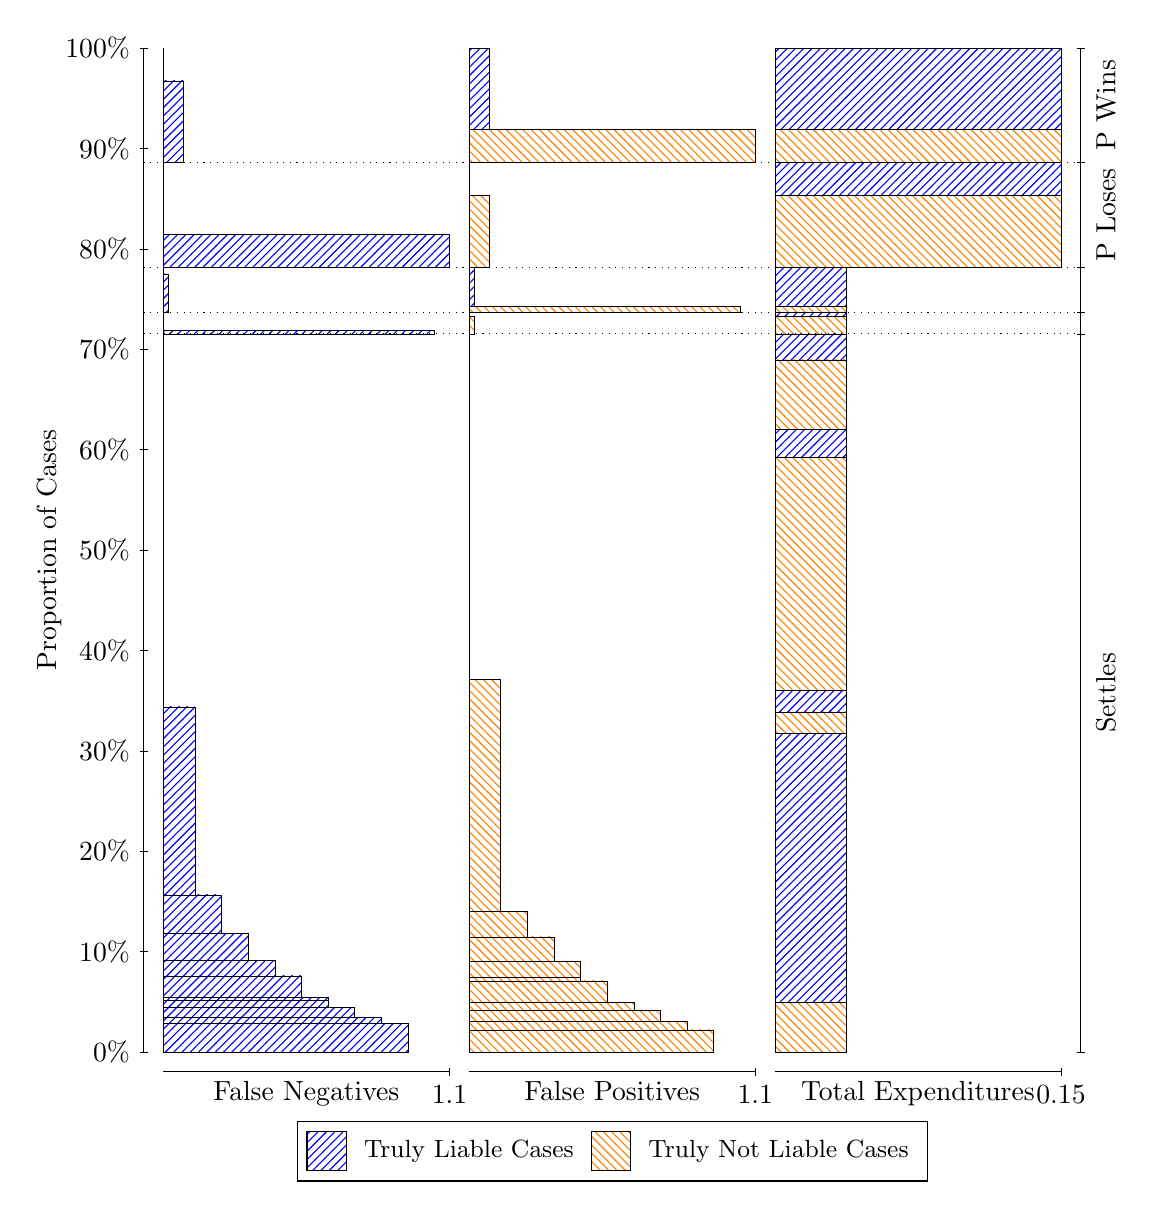
\begin{tikzpicture}
\draw[black, very thin] (1.5,1.75) -- (1.5,14.5);
\node[rotate=90, anchor=center] at (0.3, 8.125) {Proportion of Cases};
\draw[black, very thin] (1.45,1.75) -- (1.55,1.75);
\node[anchor=east] at (1.45, 1.75) {0\%};
\draw[black, very thin] (1.45,3.025) -- (1.55,3.025);
\node[anchor=east] at (1.45, 3.025) {10\%};
\draw[black, very thin] (1.45,4.3) -- (1.55,4.3);
\node[anchor=east] at (1.45, 4.3) {20\%};
\draw[black, very thin] (1.45,5.575) -- (1.55,5.575);
\node[anchor=east] at (1.45, 5.575) {30\%};
\draw[black, very thin] (1.45,6.85) -- (1.55,6.85);
\node[anchor=east] at (1.45, 6.85) {40\%};
\draw[black, very thin] (1.45,8.125) -- (1.55,8.125);
\node[anchor=east] at (1.45, 8.125) {50\%};
\draw[black, very thin] (1.45,9.4) -- (1.55,9.4);
\node[anchor=east] at (1.45, 9.4) {60\%};
\draw[black, very thin] (1.45,10.675) -- (1.55,10.675);
\node[anchor=east] at (1.45, 10.675) {70\%};
\draw[black, very thin] (1.45,11.95) -- (1.55,11.95);
\node[anchor=east] at (1.45, 11.95) {80\%};
\draw[black, very thin] (1.45,13.225) -- (1.55,13.225);
\node[anchor=east] at (1.45, 13.225) {90\%};
\draw[black, very thin] (1.45,14.5) -- (1.55,14.5);
\node[anchor=east] at (1.45, 14.5) {100\%};

\draw[black, very thin] (13.4,1.75) -- (13.4,14.5);
\draw[black, very thin] (13.35,1.75) -- (13.45,1.75);
\node[anchor=west] at (13.35, 1.75) {};
\draw[black, very thin] (13.35,10.87) -- (13.45,10.87);
\node[anchor=west] at (13.35, 10.87) {};
\draw[black, very thin] (13.35,11.139) -- (13.45,11.139);
\node[anchor=west] at (13.35, 11.139) {};
\draw[black, very thin] (13.35,11.715) -- (13.45,11.715);
\node[anchor=west] at (13.35, 11.715) {};
\draw[black, very thin] (13.35,13.046) -- (13.45,13.046);
\node[anchor=west] at (13.35, 13.046) {};
\draw[black, very thin] (13.35,14.5) -- (13.45,14.5);
\node[anchor=west] at (13.35, 14.5) {};

\draw[black, very thin, pattern color=blue, pattern=north east lines] (1.75,1.75) rectangle (4.8552,2.109);
\draw[black, very thin, pattern color=blue, pattern=north east lines] (1.75,2.109) rectangle (4.5172,2.1901);
\draw[black, very thin, pattern color=blue, pattern=north east lines] (1.75,2.1901) rectangle (4.1793,2.3185);
\draw[black, very thin, pattern color=blue, pattern=north east lines] (1.75,2.3185) rectangle (3.8413,2.4004);
\draw[black, very thin, pattern color=blue, pattern=north east lines] (1.75,2.4004) rectangle (3.8413,2.4401);
\draw[black, very thin, pattern color=blue, pattern=north east lines] (1.75,2.4401) rectangle (3.5033,2.7171);
\draw[black, very thin, pattern color=blue, pattern=north east lines] (1.75,2.7171) rectangle (3.1653,2.9091);
\draw[black, very thin, pattern color=blue, pattern=north east lines] (1.75,2.9091) rectangle (2.8273,3.257);
\draw[black, very thin, pattern color=blue, pattern=north east lines] (1.75,3.257) rectangle (2.4893,3.744);
\draw[black, very thin, pattern color=blue, pattern=north east lines] (1.75,3.744) rectangle (2.1514,6.1336);
\draw[black, very thin, pattern color=orange, pattern=north west lines] (1.75,6.1336) rectangle (1.75,10.87);
\draw[black, very thin, pattern color=blue, pattern=north east lines] (1.75,10.87) rectangle (5.1932,10.914);
\draw[black, very thin, pattern color=orange, pattern=north west lines] (1.75,10.914) rectangle (1.75,11.139);
\draw[black, very thin, pattern color=blue, pattern=north east lines] (1.75,11.139) rectangle (1.8134,11.633);
\draw[black, very thin, pattern color=orange, pattern=north west lines] (1.75,11.633) rectangle (1.75,11.715);
\draw[black, very thin, pattern color=blue, pattern=north east lines] (1.75,11.715) rectangle (5.3833,12.131);
\draw[black, very thin, pattern color=orange, pattern=north west lines] (1.75,12.131) rectangle (1.75,13.046);
\draw[black, very thin, pattern color=blue, pattern=north east lines] (1.75,13.046) rectangle (2.0035,14.083);
\draw[black, very thin, pattern color=orange, pattern=north west lines] (1.75,14.083) rectangle (1.75,14.5);
\draw[black, very thin, pattern color=orange, pattern=north west lines] (5.6333,1.75) rectangle (8.7386,2.0308);
\draw[black, very thin, pattern color=orange, pattern=north west lines] (5.6333,2.0308) rectangle (8.4006,2.1401);
\draw[black, very thin, pattern color=orange, pattern=north west lines] (5.6333,2.1401) rectangle (8.0626,2.2824);
\draw[black, very thin, pattern color=orange, pattern=north west lines] (5.6333,2.2824) rectangle (7.7246,2.3836);
\draw[black, very thin, pattern color=orange, pattern=north west lines] (5.6333,2.3836) rectangle (7.3866,2.6526);
\draw[black, very thin, pattern color=orange, pattern=north west lines] (5.6333,2.6526) rectangle (7.0486,2.6939);
\draw[black, very thin, pattern color=orange, pattern=north west lines] (5.6333,2.6939) rectangle (7.0486,2.8978);
\draw[black, very thin, pattern color=orange, pattern=north west lines] (5.6333,2.8978) rectangle (6.7107,3.2125);
\draw[black, very thin, pattern color=orange, pattern=north west lines] (5.6333,3.2125) rectangle (6.3727,3.5356);
\draw[black, very thin, pattern color=orange, pattern=north west lines] (5.6333,3.5356) rectangle (6.0347,6.4862);
\draw[black, very thin, pattern color=blue, pattern=north east lines] (5.6333,6.4862) rectangle (5.6333,10.87);
\draw[black, very thin, pattern color=orange, pattern=north west lines] (5.6333,10.87) rectangle (5.6967,11.095);
\draw[black, very thin, pattern color=blue, pattern=north east lines] (5.6333,11.095) rectangle (5.6333,11.139);
\draw[black, very thin, pattern color=orange, pattern=north west lines] (5.6333,11.139) rectangle (9.0766,11.221);
\draw[black, very thin, pattern color=blue, pattern=north east lines] (5.6333,11.221) rectangle (5.6967,11.715);
\draw[black, very thin, pattern color=orange, pattern=north west lines] (5.6333,11.715) rectangle (5.8868,12.63);
\draw[black, very thin, pattern color=blue, pattern=north east lines] (5.6333,12.63) rectangle (5.6333,13.046);
\draw[black, very thin, pattern color=orange, pattern=north west lines] (5.6333,13.046) rectangle (9.2667,13.462);
\draw[black, very thin, pattern color=blue, pattern=north east lines] (5.6333,13.462) rectangle (5.8868,14.5);
\draw[black, very thin, pattern color=orange, pattern=north west lines] (9.5167,1.75) rectangle (10.425,2.3836);
\draw[black, very thin, pattern color=blue, pattern=north east lines] (9.5167,2.3836) rectangle (10.425,5.8001);
\draw[black, very thin, pattern color=orange, pattern=north west lines] (9.5167,5.8001) rectangle (10.425,6.0691);
\draw[black, very thin, pattern color=blue, pattern=north east lines] (9.5167,6.0691) rectangle (10.425,6.3461);
\draw[black, very thin, pattern color=orange, pattern=north west lines] (9.5167,6.3461) rectangle (10.425,9.2967);
\draw[black, very thin, pattern color=blue, pattern=north east lines] (9.5167,9.2967) rectangle (10.425,9.6557);
\draw[black, very thin, pattern color=orange, pattern=north west lines] (9.5167,9.6557) rectangle (10.425,10.539);
\draw[black, very thin, pattern color=blue, pattern=north east lines] (9.5167,10.539) rectangle (10.425,10.87);
\draw[black, very thin, pattern color=orange, pattern=north west lines] (9.5167,10.87) rectangle (10.425,11.095);
\draw[black, very thin, pattern color=blue, pattern=north east lines] (9.5167,11.095) rectangle (10.425,11.139);
\draw[black, very thin, pattern color=orange, pattern=north west lines] (9.5167,11.139) rectangle (10.425,11.221);
\draw[black, very thin, pattern color=blue, pattern=north east lines] (9.5167,11.221) rectangle (10.425,11.715);
\draw[black, very thin, pattern color=orange, pattern=north west lines] (9.5167,11.715) rectangle (13.15,12.63);
\draw[black, very thin, pattern color=blue, pattern=north east lines] (9.5167,12.63) rectangle (13.15,13.046);
\draw[black, very thin, pattern color=orange, pattern=north west lines] (9.5167,13.046) rectangle (13.15,13.462);
\draw[black, very thin, pattern color=blue, pattern=north east lines] (9.5167,13.462) rectangle (13.15,14.5);
\draw[black, dotted] (1.5,10.87) -- (13.4,10.87);
\draw[black, dotted] (1.5,11.139) -- (13.4,11.139);
\draw[black, dotted] (1.5,11.715) -- (13.4,11.715);
\draw[black, dotted] (1.5,13.046) -- (13.4,13.046);
\draw[black, very thin] (1.75,1.5) -- (5.3833,1.5);
\node[anchor=north] at (3.5667, 1.5) {False Negatives};
\draw[black, very thin] (5.3833,1.45) -- (5.3833,1.55);
\node[anchor=north] at (5.3833, 1.45) {1.1};

\draw[black, very thin] (5.6333,1.5) -- (9.2667,1.5);
\node[anchor=north] at (7.45, 1.5) {False Positives};
\draw[black, very thin] (9.2667,1.45) -- (9.2667,1.55);
\node[anchor=north] at (9.2667, 1.45) {1.1};

\draw[black, very thin] (9.5167,1.5) -- (13.15,1.5);
\node[anchor=north] at (11.333, 1.5) {Total Expenditures};
\draw[black, very thin] (13.15,1.45) -- (13.15,1.55);
\node[anchor=north] at (13.15, 1.45) {0.15};

\node[black, centered, rotate=90] at (13.72, 6.3099) {Settles};


\node[black, centered, rotate=90] at (13.72, 12.38) {P Loses};
\node[black, centered, rotate=90] at (13.72, 13.773) {P Wins};

\draw (7.449999999999999,1.5) node[draw=none] (baseCoordinate) {};
\begin{scope}[align=center]
        \matrix[scale=0.5, draw=black, below=0.5cm of baseCoordinate, nodes={draw}, column sep=0.1cm]{
            \node[rectangle, draw, minimum width=0.5cm, minimum height=0.5cm, pattern=north east lines, pattern color=blue] {}; &
            \node[draw=none, font=\small] (B) {Truly Liable Cases}; &
            \node[rectangle, draw, minimum width=0.5cm, minimum height=0.5cm, pattern=north west lines, pattern color=orange] {}; &
            \node[draw=none, font=\small] (B) {Truly Not Liable Cases}; \\
            };
\end{scope}

\end{tikzpicture}
\end{document}